\documentclass[12pt]{article}

\usepackage{apacite}
\usepackage{geometry}
\geometry{letterpaper}                   
\usepackage{graphicx}
\usepackage{amssymb}
\usepackage{epstopdf}
\usepackage{amsmath}
\usepackage{hyperref}
\usepackage{comment}
\usepackage{caption}
\allowdisplaybreaks
\graphicspath{ {./Figures} }

\renewcommand{\baselinestretch}{1.1}

\setlength{\topmargin}{-0.60in} \setlength{\oddsidemargin}{-0.2in}
\setlength{\textwidth}{6.5in} \setlength{\textheight}{9in}


\def\E{{\rm E}}
\def\Var{{\rm Var}}
\def\Cov{{\rm Cov}}
\def\KL{{\rm KL}}


\begin{document}

\noindent{Ryan O'Dell} \\
\noindent{Nick Kim} \\
12/11/2021 \\
\begin{center}
{\huge Hyperparameter Tuning for Gradient Boosting Frameworks } 
\end{center}

\section{Introduction}
Experimental design is a crucial part of any statistical experiment, including computer simulations. To explore the effects of efficient design on a computer experiment, we have examined three scientific papers and repeated the papers’ experiments with our own methods of analysis using principles of design discussed in class. 

In the computer simulations discussed here, the experiments are the machine learning models themselves, with the predictive performance of the model serving as the output and the various hyperparameters serving as the inputs. A common theme throughout all the papers we examined was an expensive grid search to optimize the model parameters. However, this framework does not attempt to model or account for the relationships between the model performance and hyperparameters. We would like to address these shortcomings in our analysis. 

 For our project, we keep a few key goals in mind. First of all, we would like to achieve better predictive performance than what was reported in each of the individual papers. Secondly, we look to reduce the estimated run time. And lastly, we seek to produce a systematic framework with which we may continually improve our models performance. As for our methodology, we incorporated principles of computer experiment design in conjunction with Gaussian Process (GP) modeling.
 
In each paper, the authors used a common method: XGBoost (Chen et al. 2016). For a quick description of the model parameters see (Chen et al. 2018a). In the remainder of the of our report we discuss each research paper in turn, comparing their experimental design and results to that of our analysis. Tables and Figures for each paper appear in the Appendix at the end of our document.

\section{Critical Temperatures of Superconductors}
The first paper we will analyze is “A Data-Driven Statistical Model for Predicting the Critical Temperature of a Superconductor”, published in the \textit{Journal of Computational Material Science}. The author's objective in this first paper is to predict at which temperature a material becomes a superconductor.\footnote{A superconductor is classified as any material which can transport electric charge with no resistance or with no energy loss} A good use case for modeling this relationship is to pre-screen various compounds and find their critical temperatures. There is currently no widely accepted physical theory for the critical temperature of a superconductor, so using a statistical model is a good alternative to model the behavior.

In the dataset that the author used and provided, the outcome variable is the critical temperature and the predictor variables are various physical properties of the material, such as atomic mass, atomic radius, etc. The data has 21,263 observations in total with 82 columns.
For their analysis, the author conducted an exhaustive 198-point grid search over five hyperparameters: learning rate, column subsampling, row subsampling, minimum nodes, and maximum depth (Table 1). This amounts to taking all possible combinations of their chosen level settings. For performance evaluation, they used a 25-fold Monte Carlo cross-validation (CV) using root mean square error (RMSE) as the performance metric. For each iteration they split the data in two thirds for model fitting and one third for model evaluation.

In our analysis, we constructed a Maximum Projection Latin Hypercube with 10 data points (using the MaxPro package) and we used the same evaluation procedure as the author did.  To transform samples from our design to integers, for parameters such as number of trees and number of leaves, we applied the samples to the inverse CDF of the uniform distribution and took the ceiling of the resulting values. To transform the continuous parameters from our design into the appropriate range we simply shifted them by a linear transformation. We repeated this procedure for all three papers.

Figure 1 shows a comparison of all two-dimensional projections of the design that we generated and the design used by the author. From the plots we can see the author's design is not space filling in all projections, however our design does enjoy good space filling and projection properties. Some of the projections of the author's design are absurd, such as the max depth and min node which project as a line. Although some of the author's parameters are uniformly distributed, like maximum depth, this is not the case for all of their parameters, especially for the continuous parameters like learning rate. 

As for the Gaussian Process Model, we used the Matern (5/2) covariance function with a small noise term added and linear mean functions. We introduce the noise term due to the fact that parameters like row and column subsampling are inherently random and lead to different performance evaluation (see tables 2 and 3 for estimated GP parameters). Then we ran 10 iterations of the EGO algorithm; we can see from that after only a couple iterations, the model is performing at a lower RMSE than the author's reported value (figure 2). In the end we arrived at an entirely different set of parameters than the author did (Table 4). In this instance we were able to achieve better performance in $1/10$th of the approximate run time for the author's experiment. We estimated the author's run time by taking the average run time on our 12 core desktop computer and multiplying by the number of configurations the author used.

\section{Ground State Energies}
The second paper we will look at is "Tree-Based Machine Learning Framework for Predicting Ground State Energies of Molecules", published in the \textit{Journal of Chemical Physics}. The ground state of a quantum-mechanical system is simply its lowest energy state; in this paper, all compounds analyzed were organic compounds. A practical application of this is discovering the timeframe for a pharmaceutical drug to break down in the body. The author's data consisted of 16242 observations and 50 columns, simplified from their original data with approximately 1300 columns via principal component analysis. The data is available at the author's GitHub: \url{https://github.com/bhimmetoglu/RoboBohr}.

The author's design in this paper was very similar to what we saw in the first paper, except the level settings of the parameters are available in the GitHub repository and not directly in the paper. Additionally, they used early stopping to determine the optimal number of trees in their final model. They performed a 576-point grid search over several hyperparameters (Table 5), and for their performance evaluation they used 5-fold CV with RMSE as the metric. Since the author reported both the 5-fold CV RMSE and the test set RMSE, we compared our results with the 5-fold CV RMSE since we did not have direct access to their exact test set.

As for our design, we generated a Maximin Latin Hypercube with 25 data points (LHS package) and incorporated the number of trees as a parameter in the experiment. Similarly, we refer to the comparison of the two-dimensional projection plots (Figure 3) and see that the author's design does not enjoy space filling properties. One thing to note was that because they used early stopping we couldn't directly compare the designs for the number of trees.

For our GP model we used the same Matern covariance function with small noise term and linear mean functions (For Parameter Estimates see Table 6 and 7). This time , we ran the EGO algorithm for 15 iterations (Figure 4). We ran EGO for a few more iterations than in our first analysis simply due to the smaller run time. Again, we see that the EGO method is able to achieve better performance than what the author reported in just a few iterations. 

From the final model parameters (Table 8), we can see that most of the parameter levels were quite different; however, it is interesting to note that the minimum nodes and learning rate parameters were almost the same. In this instance we were able to achieve better performance in $1/15$th of the approximate run time for the author's experiment.

\section{Quantitative Structure-Activity Relationships}
The third paper we examined, “Extreme Gradient Boosting as a Method for Quantitative Structure–Activity Relationships” from the \textit{Journal of Chemical Information and Modeling}, concerned building a statistical model for Quantitative Structure-Activity Relationships. QSAR is a popular technique for predicting pharmaceutical drug effects and side effects. These models typically help to streamline the drug production process by helping to prioritize novel compounds in the pre-clinical trial stage based on the model predictions.

          	The paper is a survey of various methods (e.g., XGBoost, Deep Neural Networks, and Random Forests) applied to several data sets curated by the pharmaceutical company Merck. For our experiments we examined the author’s follow up paper which is a pre-print, where they extend the methods to include LightGBM. LightGBM is Microsoft's implementation of XGBoost that is a bit more memory efficient and runs faster. We chose to focus on only one of the data sets and examined the LightGBM algorithm. The data set we chose to analyze was the logD \footnote{logD is an important measurement in drug synthesis because it measures the lipophilicity of a drug} data set, where the dependent variable was the logD measurement of various compounds. In total, the data set had 50,000 rows of data for model fitting and 50,000 rows of data for model evaluation. In total, there were 8,921 independent variables used to predict the outcome.         
          	
          	To select the optimal set of parameters for their model, the authors used a sequential grid search on the following model parameters: number of trees, learning rate, number of leaves, column subsampling, and row subsampling. To perform a sequential grid search, the authors first fixed the number of leaves to 32, row subsampling to 0.70, and column subsampling to 0.70. They then fit and evaluated the model across all combinations of the number of trees with values (1500,700,350,100) and learning rate with values (0.01,0.02,0.05,0.1). The optimal set of parameters was found and then they proceeded to grid search for the number of leaves with values (16,32,64,128,256). Lastly, they grid searched for the row and column subsampling with values of (0.25,0.50,0.7,1.0). The total number of configurations run was 37 and amounted to using 3 different designs (Figures 5,6, and 7).
          	
 For model evaluation, they used 2-fold CV on the training set and then took the parameters with the best performance, fit the model to the entire training data set, and reported the R-squared value on the test set.
 
To compare, we generated a 15-point Maximum Projection Latin Hypercube with all parameters within the same parameter ranges designated by the author, except we increased the number of trees / boosting iterations to be between 1000-1500. We realized early on that a low number of trees resulted in poor test set performance. To finalize the results, we modeled the experiment with a Gaussian Process, using a linear mean function and the Matern 5/2 covariance function with small noise term (Parameter Estimates in Table 9 and 10). The EGO algorithm was run for 15 iterations (Figure 8). The parameters we selected had the lowest RMSE estimated by the two fold CV, we then fit the model with these parameters on the entire training set and calculated the R-squared on the test set. 
 
The test sample R-squared we achieved was not higher than what the author reported for the best parameter configuration suggestion by EGO (Table 11). We stipulate this was due to only using 2-fold CV to select the best set of hyper parameters. Considering the previous two papers used 5 and 25 fold CV, it would probably be best to increase the number of folds to get a more accurate out of sample RMSE estimate. To verify this, we examined the 3 lowest RMSE parameter configurations and found that one of them did indeed have better test set R-squared (Table 12). 

 
\section{Conclusions}
Overall, we have seen that for our first two papers, using formal designs for computer experiments and the EGO algorithm resulted in better performance in a fraction of the estimated time required for the author's experiments. 

One limitation of the author's approach is that in practice, one must find the hyperparameter ranges to begin with. In our analysis, we limited ourselves to using the author's stated ranges for the parameters. However, in reality, we would need to run some pre-screening experiments to narrow down the parameter ranges down. In particular, arbitrarily defining the levels for the parameters and performing a grid search leads to an experiment with poor space filling and projection properties. Additionally, the EGO method allows for exploration of parameter levels that were not explored in the initial design. Whereas a grid search only evaluates the experiment at the initial parameter levels. One consequence of this is that  discretizing continuous parameters leads to overlooking potentially better parameter levels. Most importantly, grid searching doesn't provide a framework for modeling the relationship between the experiment's configuration and the outcome. In the end there isn't a clear or systematic way to proceed after a grid search is complete to try to improve model performance. However, design of computer experiments, GP modeling, and the EGO algorithm provide a systematic way to augment and suggest better configurations.

We now have a systematic framework for optimizing the hyper parameters of gradient boosting frameworks, but there are of course many potential avenues to further explore for even more robust models. One possibility is exploring different choices for the mean and covariance functions in the GP model. Another idea is to implement the q-step ahead procedure in the EGO algorithm, which could lead to improved run time. More generally, we could also explore some different designs such as uniform projection design.  As a last step to make a fully systematic approach to hyper parameter selection we need a pre-screening process to narrow the ranges of the parameter values.

\newpage 
\section{References}

\begin{itemize}

\item Chen, T. and Guestrin, C. (2016). Xgboost: A scalable tree boosting system. https://arxiv. org/abs/1603.02754.

\item Chen, T., He, T., Benesty, M., Khotilovich, V., and Tang, Y. (2018a). xgboost: Extreme Gradient Boosting. R package version 0.6.4.1.


\item Hamidieh, K., 2018. A data-driven statistical model for predicting the critical temperature of a superconductor. Computational Materials Science 154, 346-354.


\item Himmetoglu, B. Tree based machine learning framework for predicting ground state energies of molecules, J. Chem. Phys. 145 (13) (2016) 134101, https://doi.org/10.1063/1.4964093, 10.1063/1.4964093.


\item Ke, G.; Meng, Q.; Finley, T.; Wang, T.; Chen, W.; Ma, Weidong, Ye, Q.; Liu, T.-Y. LightGBM: A Highly Efficient Gradient Boosting DecisionTree 31st Conference on Neural Information Processing Systems (NIPS 2017), Long Beach, CA, USA.

\item Sheridan, R. P., Liaw, A., \& Tudor, M. (2021). Light Gradient Boosting Machine as a Regression Method for Quantitative Structure-Activity Relationships. arXiv preprint arXiv:2105.08626.

\item Sheridan, R. P., Wang, W. M., Liaw, A., Ma, J., and Gifford, E. M. (2016) Extreme Gradient Boosting as a Method for Quantitative Structure-Activity Relationships. J. Chem. Inf. Model. 56 (12), 2353– 2360,  DOI: 10.1021/acs.jcim.6b00591


\end{itemize}

\newpage 
\section{Appendix}

\subsection{Paper 1 }



\begin{table}[!h]
 \centering
 \begin{tabular}{ | c | c |} 

 \hline
 Parameters & Levels \\
 \hline
 Learning rate &  0.010, 0.015, 0.020 \\
Column subsampling&  0.25, 0.50, 0.75 \\
Subsample ratio & 0.5 \\
Minimum nodes & 1, 10 \\
Maximum depth & 15, 16,\dots , 25 \\
 \hline 
 \end{tabular}
 \caption{Levels Settings Paper 1 }
 \end{table}


  \begin{figure}[!hbtp]
\centering
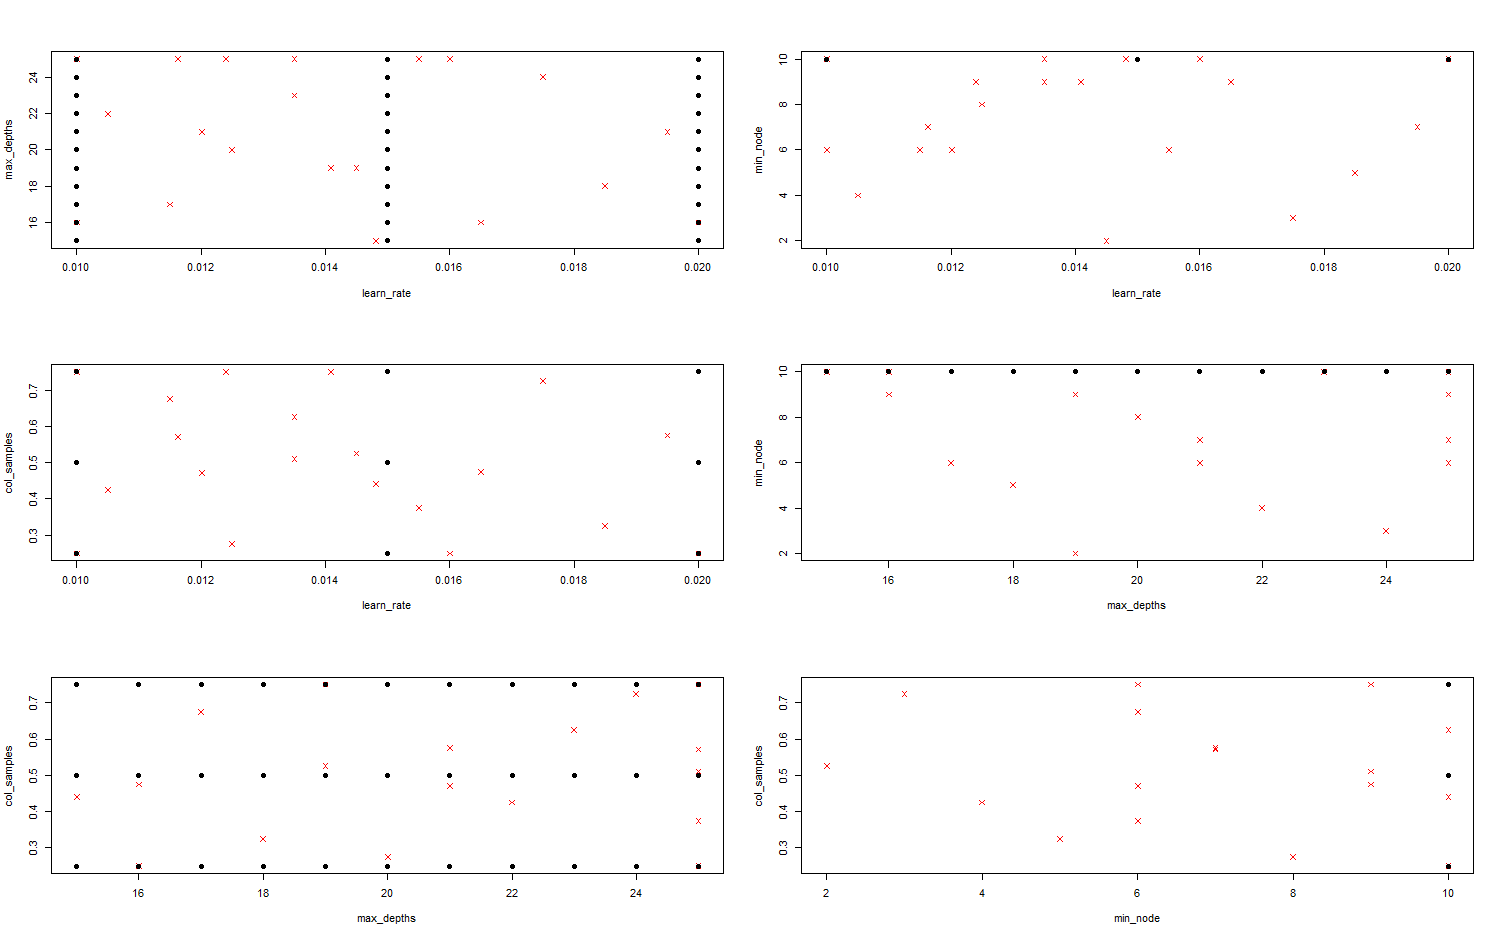
\includegraphics[scale=0.45]{paper_1_all_2D_projections.png}
\caption{ Two Dimensional Projections. Authors Design in Black. Our Design in Red.}
\end{figure}


\vspace*{2.5cm}


 
 \begin{minipage}[c]{0.5\textwidth}
 \centering
 \begin{tabular}{| c  c |} 
 \multicolumn{2}{c}{Trend  coefficient} \\

  \hline 
  Parameters & Estimates \\
 \hline 
(Intercept)   & 88.2990 \\
  learn rate  &   1.5318 \\
  max depths  &   0.4895 \\
    min node  &  -2.5596 \\
 col samples  &   0.4053 \\

 \hline
 \end{tabular}
\captionof{table}{Trend Coefficients }
\end{minipage}
\begin{minipage}[c]{0.5\textwidth}
 \centering
 \begin{tabular}{| c c |} 
 \multicolumn{2}{c}{Covariance coefficients} \\
 \hline
  Parameters &                   Estimate \\
  \hline
 theta(learn rate)   &  0.4553\\
 theta(max depths)   &  1.8000\\
   theta(min node)   &  0.1643\\
theta(col samples)  &   1.8000\\
\hline
 \end{tabular}
\captionof{table}{Variance estimate: 0.1197317}
\end{minipage}

 \vspace*{2.5cm}
 
  \begin{figure}[!hbtp]
\centering
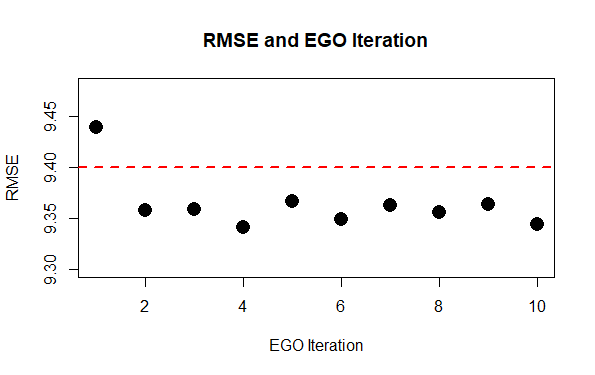
\includegraphics[scale=0.65]{super_conductor_ego.png}
\caption{EGO Progress}
\end{figure}
 

 

\begin{table}[!h]
 \centering
 \begin{tabular}{ | c | c | c |} 

 \hline
 & Papers Results & Our Results \\
 \hline
 Learning rate & 0.02 & 0.01162295 \\
Column subsampling & 0.50  & 0.57 \\
Minimum nodes & 1 & 7 \\
Maximum depth & 16 & 25 \\
RMSE & 9.4 &  9.34 \\
Estimated Time to Run & 83 hours & 8.5 hours \\
 \hline 
 \end{tabular}
 \caption{ Final Model Parameter Comparison }
 \end{table}

\newpage 

\subsection{Paper 2 }

\begin{table}[!h]
 \centering
 \begin{tabular}{ | c | c |} 

 \hline
 Parameters & Levels \\
 \hline
 Learning rate & 0.015625, 0.03125, 0.0625\\
Column subsampling &  0.2, 0.4, 0.6\\
Minimum nodes&  2, 6, 8, 10\\
Maximum depth&  2, 6, 8, 16\\
Regularization term &  0, 0.0001, 0.001, 0.01 \\
 \hline 
 \end{tabular}
 \caption{Levels Settings Paper 2 }
 \end{table}

\vspace*{2.5cm}

  \begin{figure}[!hbtp]
\centering
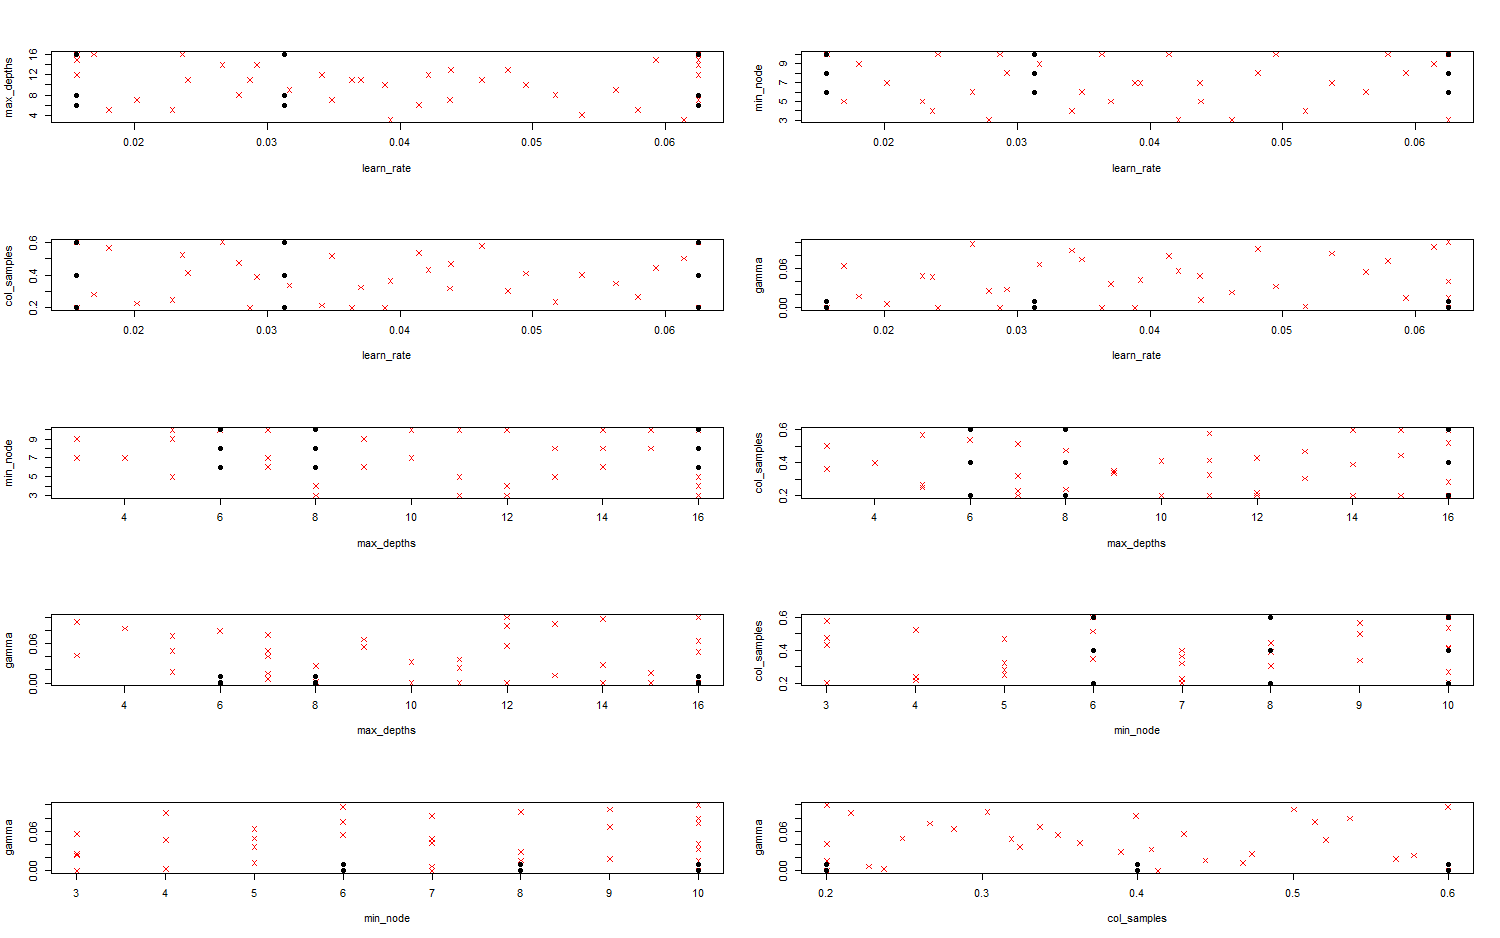
\includegraphics[scale=0.45]{paper_2_all_2D_projections.png}
\caption{Two Dimensional Projections. Authors Design in Black. Our Design in Red.}
\end{figure}




 \begin{minipage}[c]{0.5\textwidth}
 \centering
 \begin{tabular}{| c  c |} 
 \multicolumn{2}{c}{Trend  coefficient} \\
  \hline 
  Parameters & Estimates \\
 \hline 
 (Intercept) &     0.2124 \\
  learn rate  &   -0.0114\\
  max depths  &   -0.0687\\
    min node &    -0.0101\\
 col samples &     0.0063\\
       gamma &    -0.0023\\
 boost round &    -0.0167\\
 \hline
 \end{tabular}
\captionof{table}{Trend Coefficients }
\end{minipage}
\begin{minipage}[c]{0.5\textwidth}
 \centering
 \begin{tabular}{| c c |} 
 \multicolumn{2}{c}{Covariance coefficients} \\
 \hline
  Parameters &                   Estimate \\
  \hline
 theta(learn rate) &      1.7316 \\
 theta(max depths)  &    0.1184\\
   theta(min node)  &    1.4453\\
theta(col samples)  &    1.9210\\
      theta(gamma)  &    1.8976\\
theta(boost round)  &    1.6360\\

\hline
 \end{tabular}
\captionof{table}{Variance estimate: 0.0001888526}
\end{minipage}

  \begin{figure}[!hbtp]
\centering
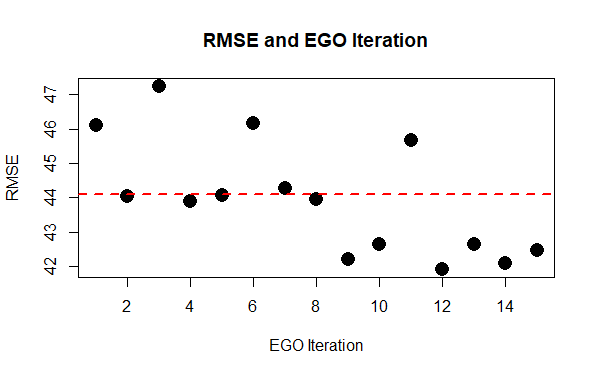
\includegraphics[scale=0.65]{ground_state_EGO.png}
\caption{EGO Progress.}
\end{figure}
 
 \vspace*{1cm}
 
\begin{table}[!h]
 \centering
 \begin{tabular}{ | c | c | c |} 

 \hline
 & Papers Results & Our Results \\
 \hline
 Learning rate & 0.0156 &0.02868557 \\
 Column subsampling & 0.40 & 0.2 \\
 Number of trees & 600 & 800 \\
 Minimum nodes & 10 & 11 \\
 Maximum depth & 16 & 10\\
Regularization term & 0.0 & 2.158121e-16 \\
RMSE & 44.09 & 41.91088 \\
Estimated Time to Run &  2 hours & 8 minutes \\

 \hline 
 \end{tabular}
 \caption{ Final Model Comparison }
 \end{table}

\newpage 
\subsection{Paper 3}



  \begin{figure}[!hbtp]
\centering
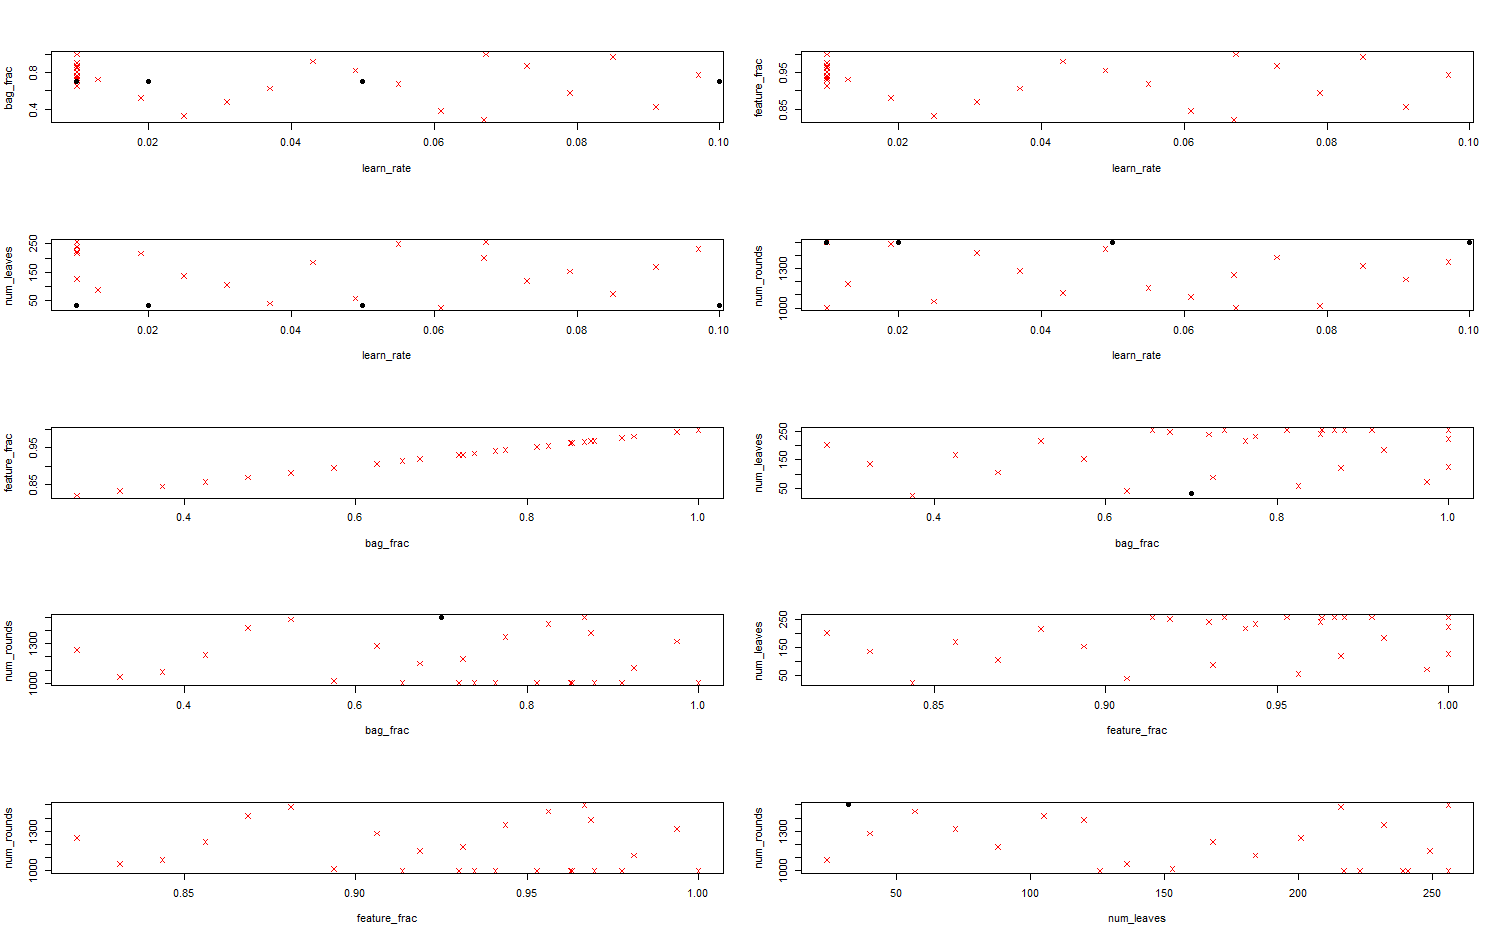
\includegraphics[scale=0.45]{paper_3_all_2D_projections_1.png}
\caption{First Grid Search over Number of Trees and Learning Rate.}
\end{figure}

\newpage

  \begin{figure}[!hbtp]
\centering
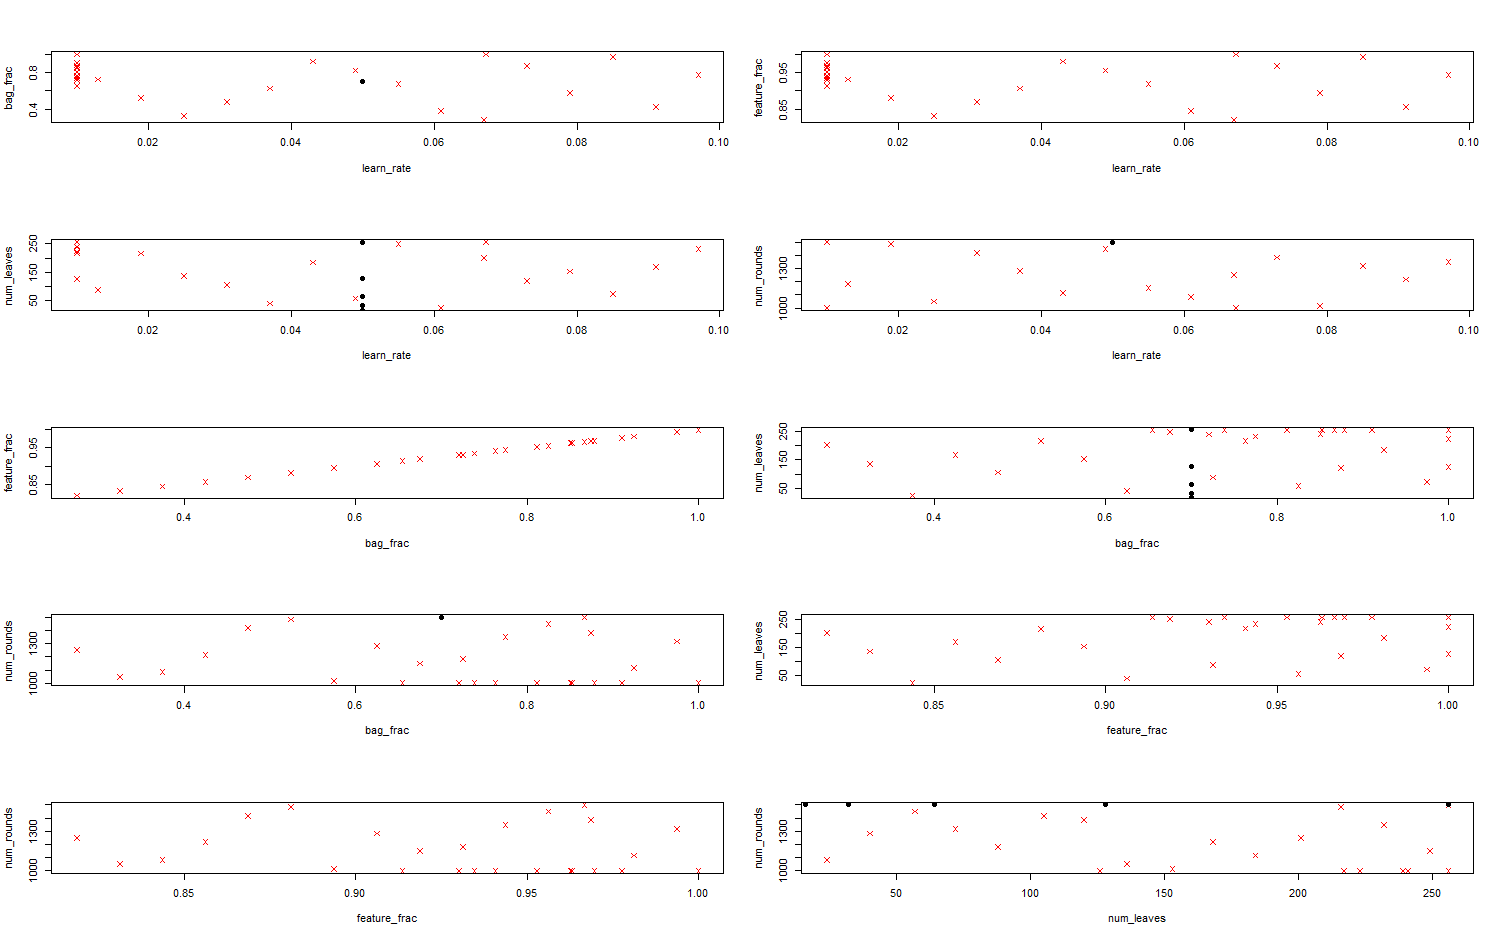
\includegraphics[scale=0.45]{paper_3_all_2D_projections_2.png}
\caption{Second Grid Search over Number of Leaves.}
\end{figure}

\newpage

  \begin{figure}[!hbtp]
\centering
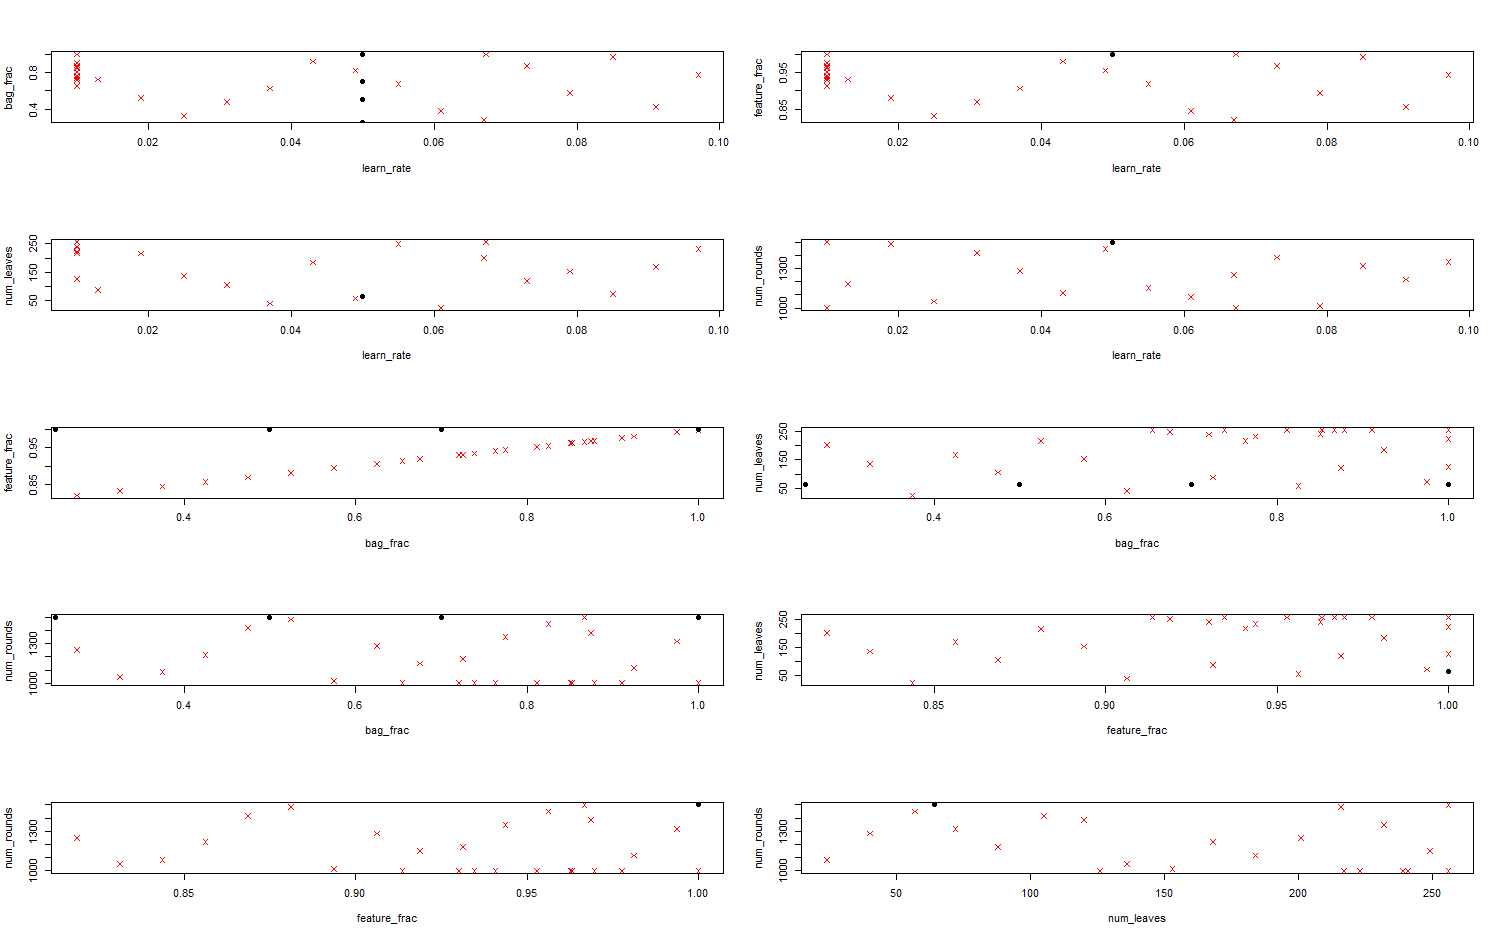
\includegraphics[scale=0.45]{paper_3_all_2D_projections_3.png}
\caption{Third Grid Search over Row and Column Sub sampling.}
\end{figure}

\vspace*{1.5cm}

 \begin{minipage}[c]{0.5\textwidth}
 \centering
 \begin{tabular}{| c  c |} 
 \multicolumn{2}{c}{Trend  coefficient} \\

  \hline 
  Parameters & Estimates \\
 \hline 
 (Intercept)  &   0.9140\\
  learn rate  &   0.0216\\
    bag frac  &  -0.0273\\
feature frac  &  -0.0012\\
  num leaves  &  -0.0268\\
  num rounds  &   0.0056\\


 \hline
 \end{tabular}
\captionof{table}{Trend Coefficients }
\end{minipage}
\begin{minipage}[c]{0.5\textwidth}
 \centering
 \begin{tabular}{| c c |} 
 \multicolumn{2}{c}{Covariance coefficients} \\
 \hline
  Parameters &                   Estimate \\
  \hline
theta(learn rate)  &   0.3812\\
    theta(bag frac)  &    0.0594\\
theta(feature frac)   &  0.3780\\
  theta(num leaves)   &  0.3670\\
  theta(num rounds)   &  0.0391\\

\hline
 \end{tabular}
\captionof{table}{Variance estimate: 2.361367e-05}
\end{minipage}



  \begin{figure}[!hbtp]
\centering
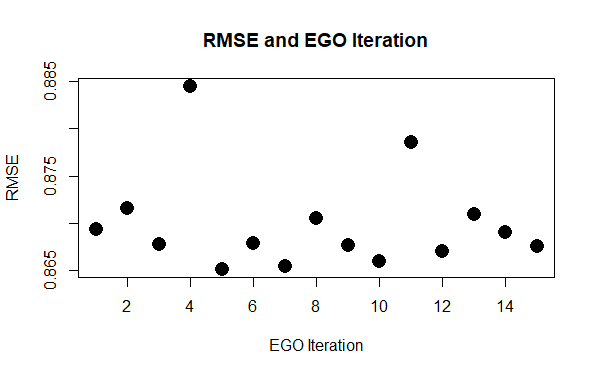
\includegraphics[scale=0.65]{QSAR_EGO.png}
\caption{EGO Progression. Performance is measured by cross validation on the training set.}
\end{figure}


\begin{table}[!h]
 \centering
 \begin{tabular}{ | c | c | c |} 

 \hline
 & Papers Results & Our Results \\
 \hline
Learning rate & 0.05 & 0.097 \\
Number of Trees &1500 &1350 \\
Column subsampling & 1 & 0.875 \\
Subsample ratio & 0.25 & 0.32 \\
Maximum leaves & 64 & 64\\
$R^{2}$ (on test data) & 0.82 & 0.81 \\
RMSE & Not reported (0.521**) & 0.526 \\
Estimated Time to Run & 15.5 Hours & 12.5 Hours \\
 \hline 
 \end{tabular}
 \caption{ Final Model Comparison }
 \end{table}
  


\end{document}